
% File acl2021.tex
%
%% Based on the style files for EMNLP 2020, which were
%% Based on the style files for ACL 2020, which were
%% Based on the style files for ACL 2018, NAACL 2018/19, which were
%% Based on the style files for ACL-2015, with some improvements
%%  taken from the NAACL-2016 style
%% Based on the style files for ACL-2014, which were, in turn,
%% based on ACL-2013, ACL-2012, ACL-2011, ACL-2010, ACL-IJCNLP-2009,
%% EACL-2009, IJCNLP-2008...
%% Based on the style files for EACL 2006 by 
%%e.agirre@ehu.es or Sergi.Balari@uab.es
%% and that of ACL 08 by Joakim Nivre and Noah Smith

\documentclass[11pt,a4paper]{article}
\usepackage[hyperref]{acl2021}

\usepackage[utf8]{inputenc}
\usepackage[T1]{fontenc}
\usepackage{todonotes}

\usepackage{times}
\usepackage{latexsym}
\renewcommand{\UrlFont}{\ttfamily\small}

% This is not strictly necessary, and may be commented out,
% but it will improve the layout of the manuscript,
% and will typically save some space.
\usepackage{microtype}

\usepackage{booktabs}
\usepackage{tabularx}
\newcolumntype{L}{>{\raggedright\arraybackslash}X}
\usepackage{svg}
\usepackage{multirow}
\usepackage{tikz}
\usepackage{amsmath}
\usepackage{natbib}
\usepackage{tabulary}

\usepackage[inline,shortlabels]{enumitem}
\newlist{lingex}{enumerate}{3} % easy numbering of examples
\setlist[lingex,1]{parsep=0pt,itemsep=1pt,label=(\arabic*),resume=lingexcount,font=\small}
\newcommand\onelingex[1]{\begin{lingex}\item #1 \end{lingex}}
\usepackage{adjustbox}

\usepackage{textcomp}
\usepackage{amssymb}

%\aclfinalcopy % Uncomment this line for the final submission
%\def\aclpaperid{***} %  Enter the acl Paper ID here

%\setlength\titlebox{5cm}
% You can expand the titlebox if you need extra space
% to show all the authors. Please do not make the titlebox
% smaller than 5cm (the original size); we will check this
% in the camera-ready version and ask you to change it back.

\newcommand\BibTeX{B\textsc{ib}\TeX}

\title{Dialogue act classification is a laughing matter}

\author{First Author \\
  Affiliation / Address line 1 \\
  Affiliation / Address line 2 \\
  Affiliation / Address line 3 \\
  \texttt{email@domain} \\\And
  Second Author \\
  Affiliation / Address line 1 \\
  Affiliation / Address line 2 \\
  Affiliation / Address line 3 \\
  \texttt{email@domain} \\}

\date{}

\begin{document}
\maketitle
\begin{abstract}
  In this paper we explore the role of laughter in attributing
  communicative intents to utterances, i.e.\ detecting the dialogue act
  performed by them. We conduct a corpus study in adult
  phone conversations showing how different dialogue acts are
  characterised by specific laughter patterns, both from the speaker
  and from the partner. Furthermore, we show that laughs can
  positively impact the performance of Transformer-based models in a
  dialogue act recognition task.  Our results highlight the importance
  of laughter for meaning construction and disambiguation in
  interaction.
  % In this paper we explore the role of laughter in interpreting the
  % meaning of an utterance, more specifically, a dialogue act performed
  % by it. We illustrate the role of laughter in pragmatic
  % disambiguation in a corpus study, and highlight the interplay
  % between non-verbal behaviours and dialogue acts performed by
  % utterances. Furthermore, we show that laughs can positively impact the
  % performance of Transformer-based models in a dialogue act recognition
  % task.
\end{abstract}


\section{Introduction}
% studies of laughter: humour, puns, functional role of laughter (Chiara), laughter prediction (Vlad)
% DAR and dialogue acts: why it is important
% gap: laughter was studied, but not when concerned with its co-locations with dialogue acts
% fill the gap:
% 1. we take a closer look, in which contexts laughter can occur w.r.t. DAs, this leads us to a hypothesis that laughter can be important for DAR
% 2. therefore, we look at laughter and its potential impact in DAR task
% 3. (we looks at non-verbals --- are they DAs?)

Laughter is ubiquitous in our everyday interactions.  In the
Switchboard Dialogue Act Corpus \citep[SWDA,][]{jurafsky1997switchboard} (US
English, phone conversations where two participants that
are not familiar with each other discuss a potentially controversial
subject, such as gun control or the school system) non-verbally vocalised
dialogue acts (whole utterances that are marked as non-verbal, 66\% of
which contain laughter) constitute 1.7\% of all dialogue acts.
Laughter tokens\footnote{Switchboard Dialogue Act Corpus does not include speech-laughs.} make up 0.5\% of all the tokens that occur in the
corpus.

Laughter relates to the discourse structure of dialogue
and can refer to a \emph{laughable}, which can be a perceived event or an
entity in the discourse.
Laughter can precede, follow or overlap the laughable, with the time
alignment between the laughter and laughable dependent on who produces
the laughable, the form of the laughter, and the pragmatic function performed \citep{tian2016we}. 
%Laughter can act as a contextual feature for determining the sincerity of an utterance, e.g. when detecting sarcasm
% \citep{tepperman2006yeah}.% ??
% VM (removed as too vague!): Some studies have already pointed out the role of laughter to disambiguate between literal or not literal interpretations of utterances.

\citet{bryant2016laughter} shows how listeners are influenced towards a non-literal interpretation of sentences when accompanied by laughter. Similarly, \citet{tepperman2006yeah} shows that laughter can act as a contextual feature for determining the sincerity of an utterance, e.g. when detecting sarcasm. % \todo{I don't know if that's ok... and I don't know if you preferred this bit here or later in the laughter background...!
% }
% VM: it is good!

Nevertheless there is a dearth of research exploring the use of
laughter in relation to different dialogue acts in detail, and
therefore little is known about the role that laughter may have in
facilitating the detection of communicative intentions.
% for Vlad! just to let you know! I noticed the "CAN" relate to a laughable ^^
% VM: what do you mean?

In this paper we investigate the disambiguation potential of laughter
for interpreting the meaning of an utterance, with the central point
being the dialogue act performed by it. To do so, we employ a
Transformer-based model and look into laughter as a potentially useful
feature for the task of \emph{dialogue act recognition} (DAR). Laughs are not
present in a large-scale pre-trained models, such as BERT \citep{Devlin2019a}, but their
representations can be learned while training for a dialogue-specific
task (DAR in our case). We further explore whether such representations
can be additionally learned, in an unsupervised fashion, from
dialogue-like data, such as a movie subtitles corpus, and if it
further improves the performance of our model. 
% Vlad check if it is right what I have written!! XD XD
% VM: perfect


The paper is organised as follows. We start with some brief background
in Section~\ref{sec:background}. In Section~\ref{sec:corpus} we
observe how dialogue acts can be classified with respect to their
collocations with laughs and discuss the patterns observed in relation
to the pragmatic functions that laughter can perform in dialogue. In
Section~\ref{sec:dar} we report our experimental results for the DAR
task depending on whether the model includes laughter. We further
investigate whether non-verbal dialogue acts can be classified as more
specific dialogue acts by our model.  We conclude with a discussion and
outlining the directions for further work in
Section~\ref{sec:discussion}.

\section{Background}
\label{sec:background}

\subsection{Laughter}
\label{sec:laughter}
%Laughter production in conversation is not exclusively related to humour. But, perhaps unsurprisingly, the study of laughter has often been linked to the study of humour and the two terms are frequently used interchangeably. However, 
% Laughter does not occur only in
% response to humour or in order to frame it. Many studies,
% particularly in conversation analysis, have shown the role of laughter in
% managing conversations at several levels: dynamics (turn-taking and
% topic-change), lexical (signalling problems of lexical retrieval or
% imprecision in the lexical choice), pragmatic (marking irony,
% disambiguating meaning, managing self-correction) and social
% (smoothing and softening difficult situations or showing
% (dis)affiliation)
% \citep{glenn2003laughter,jefferson1984organization,mazzocconi2019phd,petitjean2015laughing}.
Laughter does not occur only in
response to humour or in order to frame it. It is crucial in managing conversations in terms of dynamics (turn-taking and
topic-change), at the lexical level (signalling problems of lexical retrieval or
imprecision in the lexical choice), but also at a pragmatic (marking irony,
disambiguating meaning, managing self-correction) and social level (smoothing and softening difficult situations or showing
(dis)affiliation)
\citep{glenn2003laughter,jefferson1984organization,mazzocconi2019phd,petitjean2015laughing}.

Moreover \citet{romaniuk2009clinton} and \citet{ginzburg2020laughter}
discuss how laughter can answer or decline to answer a question, and
\citet{mazzocconi2018laughter} discusses how even isolated laughter
can be the object of clarification requests, signalling the need for
interlocutors to clarify its meaning (e.g., in terms of what the
``laughable'' is) in order to continue the conversation.

% \textcolor{blue}{<-- this is really badly written!}
%\todo{^^ I think I'll rephrase it later!! XD I've copied and pasted these sentences in way to many places already!!! XD XD XD }

%\todo{Ah! I see now the comment! Yes! I was just about to ask you if you would agree if I say a bit about the role of laughter for expliciting/disambiguating intentions! I mean... there is not much specifically speaking explicitely about laughter and dialogue acts but quite a bit I can say about the role laughter can have to disambiguate communicative intentions! }

% Chiara: is there something more related to DAs?..

\subsection{Dialogue act recognition}
\label{sec:dial-act-recogn}

The concept of a dialogue act (DA) is based on that of the speech act
\citep{austin1975things}. %CH 2009??? Not 1975? 
Breaking with classical semantic
theory, Speech Act Theory considers not only the propositional content
of an utterance but also the actions, such as \emph{promising} or
\emph{apologising}, it carries out.  Dialogue acts extend the concept
of the speech act, with a focus on the interactional nature of most
speech.  DAMSL \citep{coreCodingDialogsDAMSL1997}, for example, is an
influential DA tagging scheme where DAs are
defined in part by whether they have a \emph{forward-looking} function
(expecting a response) or \emph{backward-looking} function (in
response to a previous utterance).

Dialogue act recognition (DAR) is the task of labelling utterances with
the dialogue act they perform, given a set of dialogue act tags.  As
with other sequence labelling tasks in NLP, some notion of context is
helpful in DAR.  One of the first performant machine learning models
for DAR was a Hidden Markov Model that used various lexical and
prosodic features as input \citep{stolckeDialogueActModeling2000}.

Recent state-of-the-art approaches to dialogue act recognition
have used a hierarchical approach, using large pre-trained language models like BERT to represent utterances, and adding some representation of discourse context at the dialogue level \citep[e.g.,][]{Ribeiro2019,mehriPretrainingMethodsDialog2019}.
However \citet{darbert} observe that without fine-tuning,
standard BERT representations perform very poorly on dialogue,
even when paired with a discourse model,
suggesting that certain utterance-internal features missing
from BERT's textual pre-training data (such as laughter) 
may have an adverse effect on dialogue act recognition.

% Bill: what’s the state-of-the-art? + refer to our IWCS paper



\section{Laughs in the Switchboard Dialogue Act Corpus}
\label{sec:corpus}

In this section we analyse dialogue acts in the Switchboard Dialogue Act
Corpus according to their collocation with laughter and provide some
qualitative insights based on the statistics.

SWDA is tagged with a set of 220 dialogue act tags which, following
\citet{jurafskySwitchboardSWBDDAMSLShallowDiscourseFunction1997a}, we
cluster into a smaller set of 42 tags.

The distribution of laughs in different dialogue acts has a rather
uniform shape with a few outliers (Figure~\ref{fig:box-swda}). The
most distinct outlier is the \emph{Non-verbal} dialogue act which is
misleading with respect to laughter, because utterances only
containing a single laughter token fall into this category. However
isolated laughs can serve, for example, to acknowledge a statement, to
deflect a question, or to show appreciation
\citep{mazzocconi2019phd}. We will further conjecture on this class of
DAs in Sec.~\ref{sec:laughter-as-non}.
%is it to much if I put making a statement? too much commintment to the propositional content thingy right?! XD

\subsection{Method}
\label{sec:method}

\begin{figure}
    \fontsize{8}{10}\selectfont
  \includesvg[width=\linewidth]{img/box-swda}
  \caption{Box plots for proportions of dialogue acts which contain laughs in SWDA. On the left: proportion of DAs containing laughter, on the right: proportion of DAs having laughter in one of the adjacent utterances.}%CH: Is it justified to combine preceding and following laughters in the same plot given the differences highlighted later?
  \label{fig:box-swda}
\end{figure}

Let us illustrate our comparison schema using the other two outliers,
\emph{Downplayer} (make up 0.05\% of all utterances) and \emph{Apology} (0.04\%), comparing them with the most common dialogue
act in SWDA---\emph{Statement-Non-Opinion} (33.27\%).  We take into consideration five
laughter-related dimensions of an utterance, and create 5-dimensional
(pentagonal) representations of DAs according to them. Each
dimension's value is equal to the proportion of utterances of a given
type which contain laughter:
\begin{itemize}
\item[$\uparrow$] current utterance;
\item[$\nwarrow$] immediately preceding utterance by the same speaker;
\item[$\nearrow$] immediately following utterance by the same speaker;
\item[$\swarrow$] immediately preceding utterance by the other speaker;
\item[$\searrow$] immediately following utterance by the other speaker.
\end{itemize}

\begin{figure}
  \includegraphics[width=\linewidth]{img/orbit-apology.pdf}
  \caption{Comparison between the pentagonal representations of laughter collocations of dialogue acts.}
  \label{fig:orbit}
\end{figure}



For instance, \ref{ex:apology-downplayer} is an illustrative example
of the phenomenon shown in Figure \ref{fig:orbit}.


\begin{lingex}%CH What are # ?
\item\label{ex:apology-downplayer}\footnote{Overlapping material is marked wish hash signs.}
  \small
  \adjustbox{valign=t}{
    % \setlength\tabcolsep{1.5pt}
    \begin{tabulary}{\linewidth}{@{}>{\bf}lJ>{\em}r@{}}
      A: & I'm sorry to keep you waiting \#<laughter>.\# & Apology \\
      B: & \#Okay\# <laughter>. / & Downplayer \\
      A: & Uh, I was calling from work  & Statement (n/o) \\
\end{tabulary}}
\end{lingex}

We show the representations of all dialogue acts on
Figure~\ref{fig:da-orbits}. We believe that such a depiction helps
the reader form impressions about similarities  between
DAs based on their laughter collocations and notice the ones
that stand out in some respects.

\begin{figure*}[h!]
  \centering
  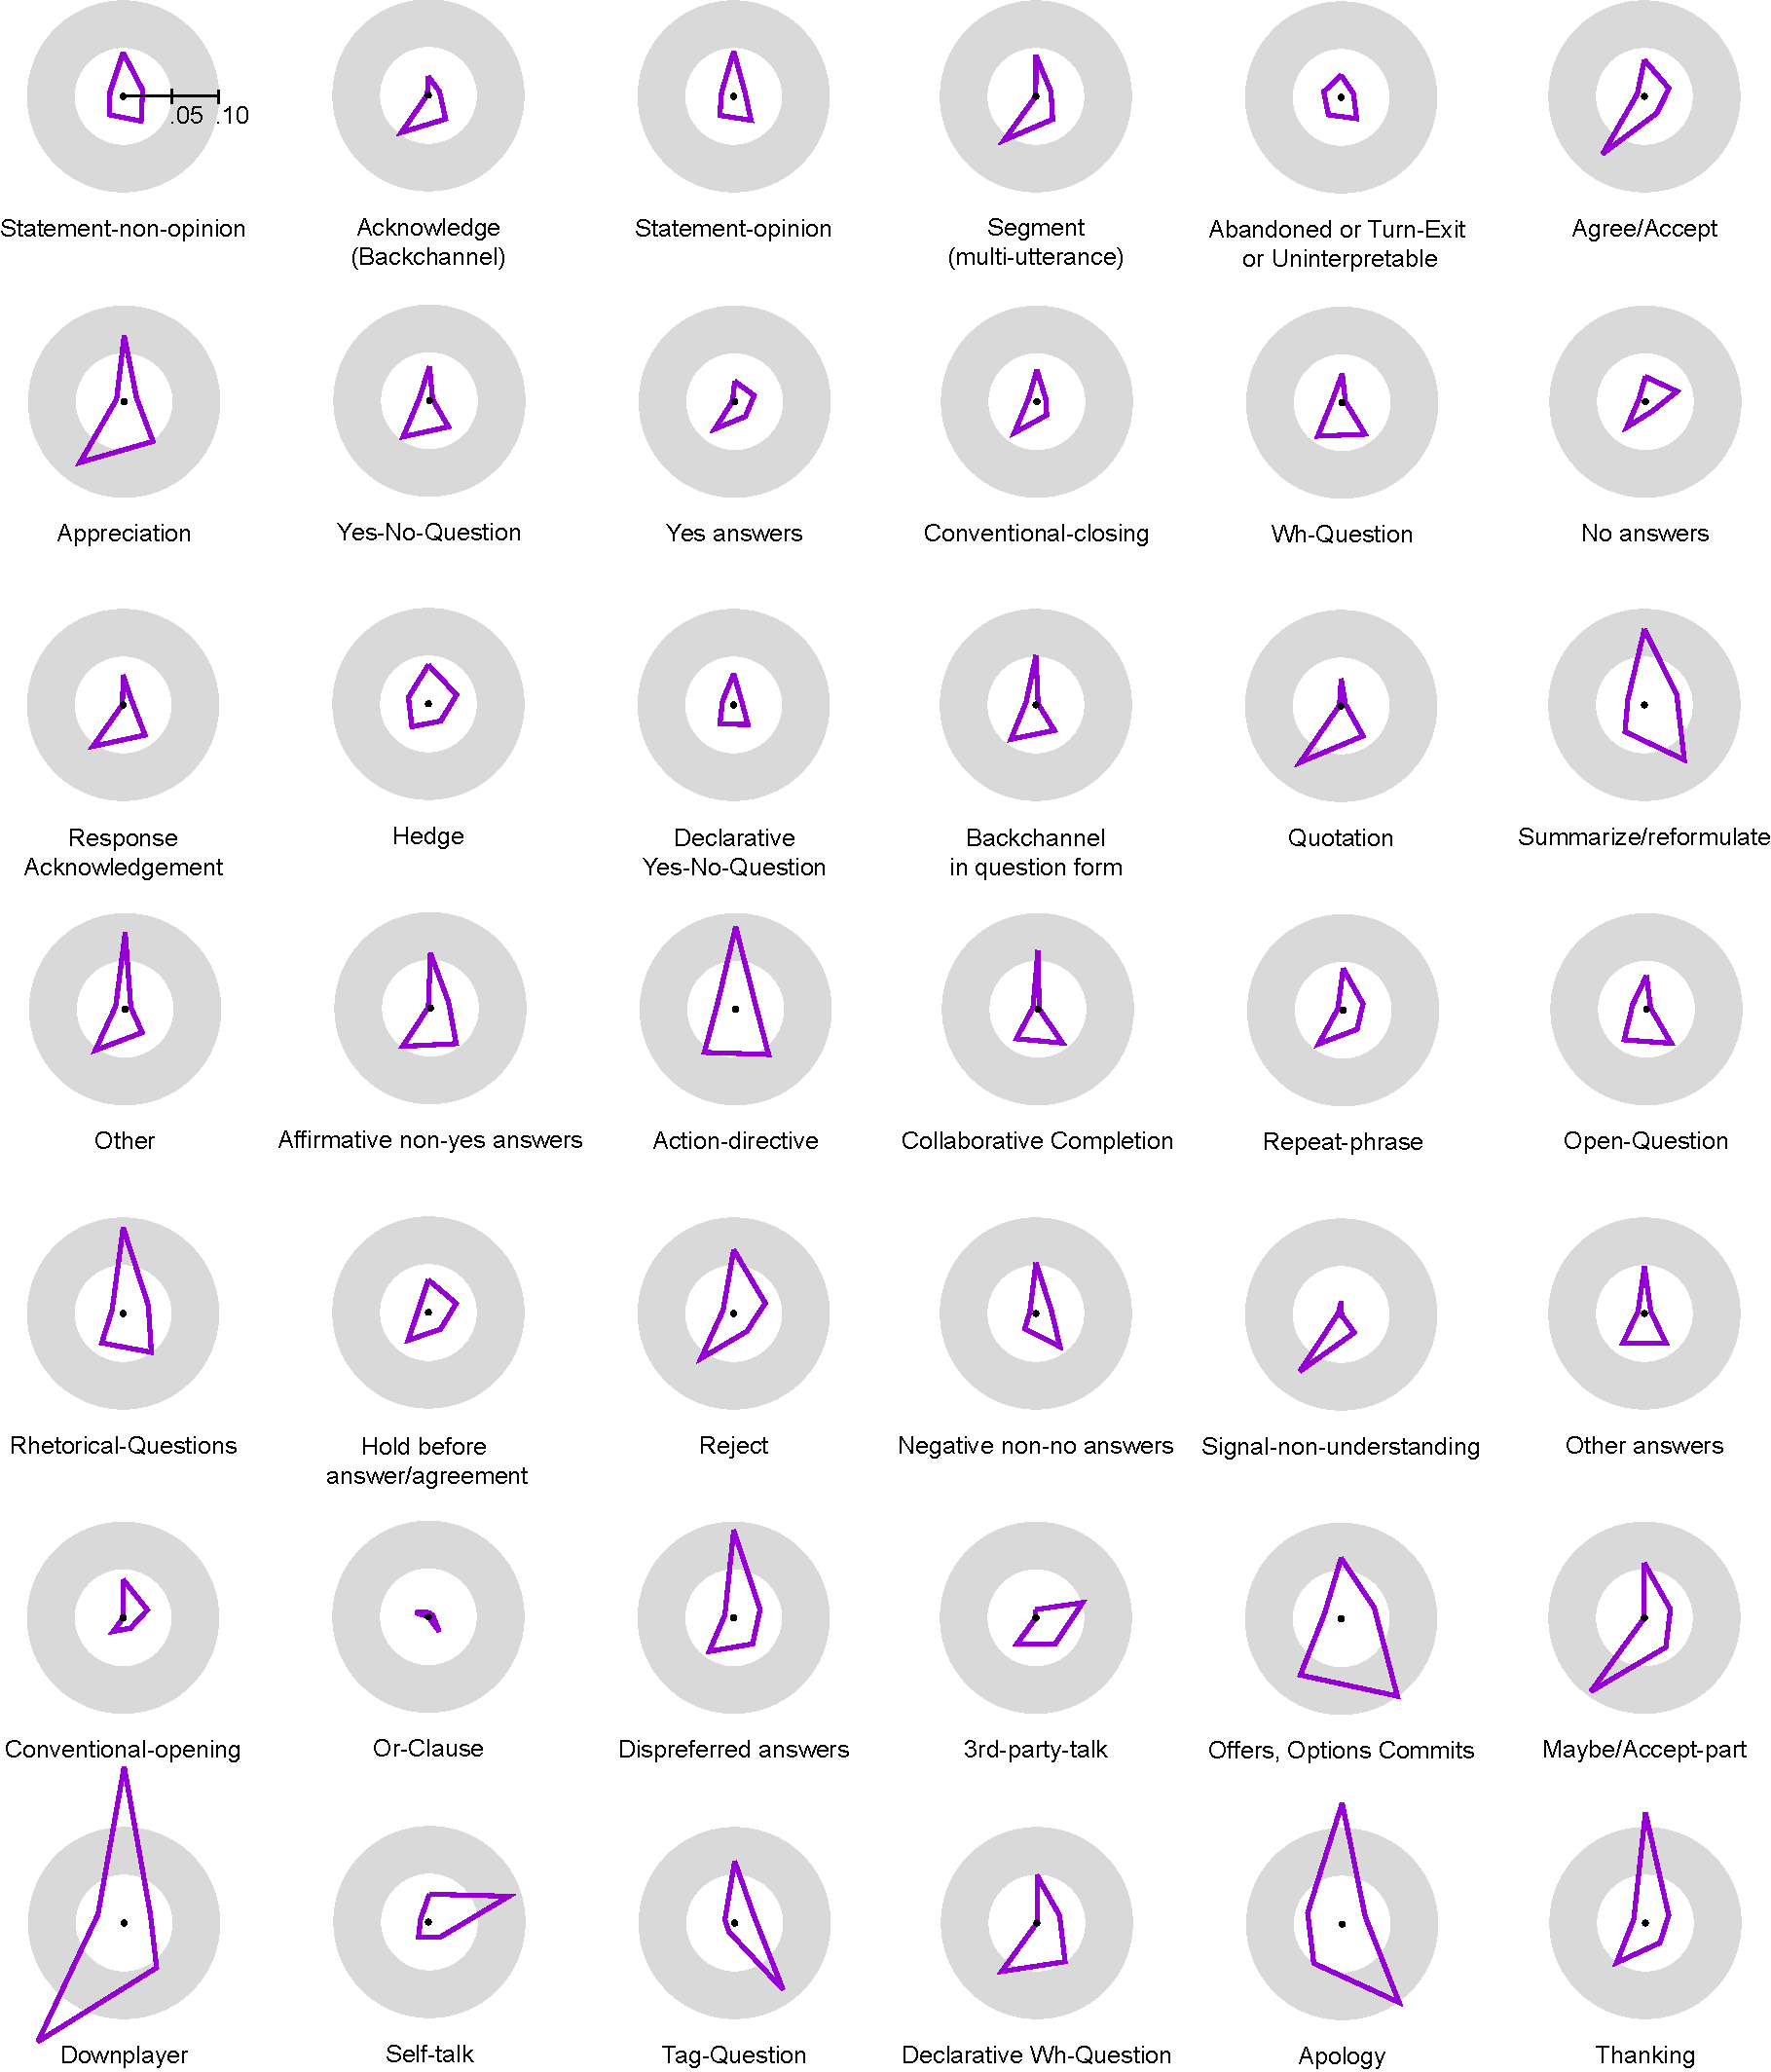
\includegraphics[width=\linewidth]{img/multiorbit.pdf}
  \caption{Pentagonal representation of dialogue acts: proportions of utterances which include laughter. Dimensions:
$\uparrow$ current utterance;
$\nwarrow$ immediately preceding utterance by the same speaker;
$\nearrow$ immediately following utterance by the same speaker;
$\swarrow$ immediately preceding utterance by the other speaker;
$\searrow$ immediately following utterance by the other speaker.
DAs are ordered by their frequency in SWDA (left-to-right, then top-to-bottom).
    \label{fig:da-orbits}}
\vspace*{-0.5cm}
\end{figure*}

To further assess the similarity between dialogue acts based on their
collocations with laughs we factorise their pentagonal representations
into 2D space using singular value decomposition (SVD). We can see
that dialogue acts form some distinct clusters.
% TODO: CH's note
The resulting plot is
shown in Figure~\ref{fig:da-svd} in Appendix~\ref{sec:app:da-svd}. Let
us now proceed with some qualitative observations.


\subsection{Observations}
\label{sec:observations}
\paragraph{Laughter and modification or enrichment of the current DA}
We observe a higher proportion of laughter accompanying the current
dialogue act ($\uparrow$) when the laughter is aimed at modifying
the current dialogue act with some degree of urgency in order to
smooth or soften it (\emph{Action-directive}, \emph{Reject},
\emph{Dispreferred answer}, \emph{Apology}), to contribute to its
enrichment stressing the positive disposition towards the partner
(\emph{Appreciation}, \emph{Downplayer}, \emph{Thanking}), or to cue
for the need to consider a less probable meaning, therefore helping
in non-literal meaning interpretation (\emph{Rhetorical question}).
 
While \emph{Apology} and \emph{Downplayer} have rather distinct and peculiar
patterns (Fig.~\ref{fig:da-svd}) discussed in more detail below, we
observe \emph{Dispreferred answers}, \emph{Action directives},
\emph{Offers/Options/Commits} and \emph{Thanking} to constitute a
close cluster when considering the decomposed values of the pentagonal
used for DA representation.%CH ??? I don't understand this sentence!
 
\paragraph{Laughter for benevolence induction and laughter as a response}
The patterns observed in relation to the preceding and following
turns reflect the multitude of functions that
laughter can perform in interaction, stressing the fact that it can be
used both to induce or invite a determinate response (dialogue act) from
the partner (\emph{Downplayer}, \emph{Agree/Accept}, \emph{Appreciation}, \emph{Acknowledge})
as well as being a possible answer to specific dialogue acts
(e.g. \emph{Apology}, \emph{Offers/Options/Commits}, \emph{Summarise/Reformulate},
\emph{Tag-question}).

A peculiar case is than the one of \emph{Self-talk}, often followed by
laughter by the same speaker. In this case the laughter may be
produced to signal the incongruity of the action (in dialogue we
normally speak to others, not to ourselves), while at the same time
function to smooth the situation, for instance, when having issues of
lexical retrieval, as in \ref{ex:selftalk}, or some degree of
embarrassment from the speaker, when questioning whether a
contribution is appropriate or not, as in
\ref{ex:appropriate}.


% A[\%]: {F Oh, } what can, - /
% A[t1]: what is his name <lipsmack>.  /
% A[ba]: {F Oh, } durn <laughter>,  /

\begin{lingex}
\item\label{ex:selftalk}
  \small
  \adjustbox{valign=t}{
    % \setlength\tabcolsep{1.5pt}
    \begin{tabulary}{\linewidth}{@{}>{\bf}lJ>{\em}r@{}}
      A: & Have, uh, really, - &  \\
      A: & what's the word I'm looking for, & Self-talk \\
      A: & I'm just totally drawing a blank <laughter>. & Statement (n/o) \\
     
\end{tabulary}}

\item\label{ex:appropriate}
  \small
  \adjustbox{valign=t}{
    % \setlength\tabcolsep{1.5pt}
    \begin{tabulary}{\linewidth}{@{}>{\bf}lJ>{\em}r@{}}
      B: &  Well,  I don't have a Mexi-, - & Statement (n/o) \\
      B: & I don't, shouldn't say that, & Self-talk \\
      B: & I don't have an ethnic maid <laughter>. & Statement (n/o) \\
     
\end{tabulary}}
\end{lingex}


% A[+]: Have, {F uh, } really, - /
% A[t1]: what's the word I'm looking for,  /
% A[sd]: I'm just totally drawing a blank <laughter>. /

% A[\%]: {C And, } {F uh, } cold foo-, {F um, } - /
% A[t1]: what's it called,  /
% A[sd]: I forgot, <laughter>, what it's called, /
% ----

% A[sd]: {D Well, } I don't know T V shows,  /
% A[t1]: what can I tell you, {F um, }  /
% A[sv]: basically junk that's on television <laughter>. -/

% B[sd]: {D Well, } I don't have a Mexi-, - /
% B[t1]: I [ don't, + ] shouldn't say that,  /
% B[sd]: I don't have an ethnic maid <laughter>. /

% Ex. reject
% B[sv]: {C So } I'm old <laughter>. /
% A[ar]: No,  /
% A[sv]: you're not old <laughter>. /




\paragraph{Apology and Downplayer}\label{subs:ap-down}
It is interesting to comment on the parallelisms of laughter usage
in relation to \textit{Apology} and \textit{Downplayer}, represented
in Fig. \ref{fig:orbit} in contrast to \emph{Statement-non-opinion}, in
as much as their graphic representations are more or less mirror-images of each other
 and show how the dialogue acts are 
linked by the pragmatic functions laughter can perform in dialogue.

In both \textit{Apology} and \textit{Downplayer} we observe a rather
higher proportion of occurrences in which the dialogue act is
accompanied by laughter ($\uparrow$) in comparison to other DAs
(Fig. \ref{fig:da-orbits}). In the case of \textit{Apology}, laughter
can be produced to induce benevolence from the partner
\citep{mazzocconiTAC}, while in the case of \textit{Downplayer} the
laughter can be produced to reassure the partner about some situation
that had been appraised as discomforting (classified as \emph{social
incongruity} by \citealp{mazzocconiTAC}) and somehow signal that the
issue should be regarded %\todo{is declined a technical term here? If not I might swap with ``regarded''} 
as not important
\citep{romaniuk2009clinton,gazelaughter}, as in \ref{ex:socInc}.

\begin{lingex}
\item\label{ex:socInc}
  \small
  \adjustbox{valign=t}{
    % \setlength\tabcolsep{1.5pt}
    \begin{tabulary}{\linewidth}{@{}>{\bf}lJ>{\em}r@{}}
      A: & I don't, I don't think I could do that <laughter>. \# & Statement (n/o) \\
      B: & Oh, it's not bad at all. & Downplayer \\
      A: &  It's, it's a beautiful drive.  & Statement (n/o)\\
\end{tabulary}}
\end{lingex}

The interesting mirror-image %specular\todo{does it work in english? BN: I didn't know this word before but I think so? CH: I have no idea what it means. Can we rephrase so it's understandable to mere mortals??}
patterns
observable in the lower part of the graph can therefore be explained
by considering the relation between the two dialogues acts.  We
observe cases in which an \textit{Apology} is accompanied by a
laughter, and then followed by a \textit{Downplayer}, showing 
that the laughter’s positive effect was attained and successful. This
allows us to explain both the bottom left spike ($\swarrow$) observed for
\textit{Downplayer} (often preceded by an utterance by the
partner containing laughter) and the bottom right spike ($\searrow$) observed
for \emph{Apology} (often followed by an utterance by the
partner containing laughter). In example \ref{ex:apology-downplayer}
both the apology and the downplayer are accompanied by laughter, while
in \ref{ex:sorry} a typical example of a laughter accompanying an \emph{Apology}
is followed by a \emph{Downplayer}.


\begin{lingex}
\item\label{ex:sorry}
  \small
  \adjustbox{valign=t}{
    % \setlength\tabcolsep{1.5pt}
    \begin{tabulary}{\linewidth}{@{}>{\bf}lJ>{\em}r@{}}
      B: & I'm sorry <laughter>. \# & Apology \\
      A: & That's all right.  / & Downplayer \\
      B: & You,  you were talking about, uh, uh,    & Summarise\\
\end{tabulary}}
\end{lingex}

We now turn to the question of whether our qualitative observations of patters between laughs and dialogue acts can be used to improve a dialogue act recognition task.


% E.g. social inc in general

% B[sd]: [ I don't, + I don't ] think I could do that <laughter>. /
% A[bd]: {F Oh, } it's not bad at all.  /
% A[sd]: [  It's, + it's ] a beautiful drive. /

% A[sd]: I hope you can understand what I s-, \# <laughter>. \# -/
% B[bd]: \# That's okay <laughter>. \#  /
% B[sd]: I got the dryer going --

% E.g. pair apology downplayer
% B[fa]: I'm sorry <laughter>. /
% A[bd]: That's all right.  /
% A[bf]: [ You, + you ] were talking about, {F uh, } {F uh, } --

% A[fa]: I'm sorry to keep you waiting \# <laughter>. \# /
% B[bd]: \# Okay \# <laughter>. /
% A[sd]: {F Uh, } I was calling from work  /

% A[fa]: I'm sorry <laughter>. /
% B[bd]: That's okay.  /
% B[sd]: I'm Bill from Raleigh. /

% A[fa]: {D Well, } I'm sorry <laughter>. /
% B[bd]: That's okay. /
% A[qy]: {F Uh, } did you ever go to Texins at all  when you were working for T I?  /

% A[fa]: {C And } I'm sorry <laughter>. /
% B[bd]: {F Oh, } no. /
% A[sd]: We're just not real big movie goers. /


%of course these are too many examples, but we can choose! ; ) 

%  by and bd "sYmpathy" and "Downplayers" of sympathy and compliments
%These are subtypes of BACKWARDS-ATTITUDE which express not just acknoweldge or understanding, but also further emotional involvement.

% by   A.44 utt1:  I'm real sorry. /
% Actual apologies (for doing something), as opposed to markers of sympathies, are tagged as "fa", see above.

% bd is any downplayer that speakers use to respond to apologize.

% bd   B.45 utt1:  That's all right. /
% Downplayers are also used to respond to compliments.

%
% \paragraph{action-directive}
% \paragraph{summarise/reformulate }

% \paragraph{agree/accept, appreciation}



% \end{itemize}

% \begin{table}[htbp]
%       \small
%   \centering
%   \begin{tabularx}{\linewidth}{llL}
%     \toprule
%     Speaker & DA & Utterance \\ \midrule
%     A	&Apology	& I'm sorry to keep you waiting \#\texttt{<laughter>}.\#  \\
%     B &Downplayer & \#Okay\# \texttt{<laughter>}. \\
%     A	&sd	& Uh, I was calling from work  \\
%     \bottomrule
%   \end{tabularx}
%   \caption{Example from the SWDA corpus (TODO:SW???). Dialogue acts:
%     \emph{sd}---Statement-non-opinion. Overlapping material is marked
%     with hash signs. }
%   \label{tab:ex:apology-downplayer}
% \end{table}

% \item Agree/accept + Appreciation

\section{The importance of laughter in artificial dialogue act recognition}
\label{sec:dar}

% TODO motivation

\subsection{Data}\label{sec:data}
We perform experiments on the Switchboard Dialogue Act Corpus (SWDA,
42 dialogue act tags), which is a subset of the larger Switchboard
corpus, and the dialogue act-tagged portion of the AMI Meeting Corpus
(AMI-DA).  AMI uses a smaller tagset of 16 dialogue acts
\citep{GuidelinesDialogueAct2005}.

% TODO add laughter numbers for AMI!

\begin{table}[ht]
\small
\centering
\begin{tabular}{@{}ll@{}}
\textbf{Switchboard}       & \textbf{AMI Corpus}                     \\\hline
Dyadic                     & Multi-party                             \\
Casual conversation        & Mock business meeting                   \\
Telephone                  & In-person \& video                      \\
English                    & English                                 \\ 
Native speakers            & Native \& non-native speakers           \\ 
%  early '90s                 & 2000s                                   \\
2200 conversations         & 171 meetings                            \\
  \hspace{1em} 1155 in SWDA               & \hspace{1em} 139 in AMI-DA                           \\
400k utterances             & 118k utterances                         \\
  3M tokens                  & 1.2M tokens                             \\
\end{tabular}  
\caption{Comparison between Switchboard and the AMI Meeting Corpus
  \label{table:corpora}}
\end{table}

\paragraph{Preprocessing}

We make an effort to normalise transcription conventions across SWDA and AMI.
We remove disfluency annotations and slashes from the end of utterances in SWDA.
In both corpora, acronyms are tokenised as individual letters. 
All utterances are lower-cased.

Utterances are tokenised using a word piece tokeniser \citep{Wu2016} with a vocabulary of 30,000.
We add a special laughter token to the vocabulary and map all transcribed laughter to that token.
We also  prepend each utterance with a speaker token that uniquely identifies the corresponding speaker within that dialogue.


\subsection{The model}
\label{sec:model}
To test the effectiveness of BERT for DAR, we employ a simple neural architecture with two components: an encoder that vectorises utterances, and a sequence model that predicts dialogue act tags from the vectorised utterances (Figure~\ref{fig:model-architecture}).
Since we are primarily interested in comparing different utterance encoders, we use a basic RNN as the sequence model in every configuration.\footnote{We have experimented with LSTM as the sequence model, but the accuracy was not significantly different compared to RNN. It can be explained by the absence of longer distance dependencies on this level of our model.} 
The RNN takes the encoded utterance as input at each time step,
and its hidden state is passed to a simple linear classification layer over dialogue act tags.
Conceptually, the encoded utterance represents the context-agnostic features of the utterance, and the hidden state of the RNN represents the full discourse context.

\begin{figure*}
  
\tikzstyle{rnn}=[rectangle,
  thick,
  minimum height=0.5cm,
  minimum width=2cm,
  fill=cyan]
\tikzstyle{encoder}=[rectangle,
  thick,
  minimum height=0.5cm,
  minimum width=2cm,
  fill=yellow]

\centering
\begin{tikzpicture}[>=latex,text height=1.5ex,text depth=0.25ex]
  \matrix[row sep=0.5cm,column sep=0.5cm] {
  % First line: Output labels
  \node (Y_0) []{$\hat{Y}_0$};&
  \node (Y_1) []{$\hat{Y}_1$};&
  \node (dots1) [] {$\dots$};  &
  \node (Y_T) []{$\hat{Y}_T$};&
  \\ % Second line: RNNs
  \node (RNN_0) [rnn]{RNN};&
  \node (RNN_1) [rnn]{RNN};&
  \node (dots2) [] {$\dots$};  &
  \node (RNN_T) [rnn]{RNN};&
  \\ % Third line: Linear layers
  \node (Encoder_0) [encoder]{Encoder};&
  \node (Encoder_1) [encoder]{Encoder};&
  \node (dots3) [] {$\dots$};  &
  \node (Encoder_T) [encoder]{Encoder};&
  \\ % Fourth line: Linear layers
  \node (Input_0) []{\small $ \underbrace{s^0,w^0_{0},w^0_{1},...,w^0_{n_0}}_{\text{Utterance 1}}$};&
  \node (Input_1) []{\small $ \underbrace{s^1,w^1_{0},w^1_{1},...,w^1_{n_1}}_{\text{Utterance 2}}$};&
  \node (dots4) [] {$\dots$};  &
  \node (Input_T) []{\small $ \underbrace{s^T,w^T_{0},w^T_{1},...,w^T_{n_T}}_{\text{Utterance T}}$};&
  \\ };
  \path[->]
  (Input_0) edge[thick]  (Encoder_0)	
  (Input_1) edge[thick] (Encoder_1)	
  (Input_T) edge[thick] (Encoder_T)	

  (Encoder_0) edge[thick] node[right] {} (RNN_0)	
  (Encoder_1) edge[thick] node[right] {} (RNN_1)	
  (Encoder_T) edge[thick] node[right] {} (RNN_T)	

  (RNN_0) edge[thick] (Y_0)	
  (RNN_1) edge[thick] (Y_1)	
  (RNN_T) edge[thick] (Y_T)	

  (RNN_0) edge[thick] node[above] {$h_1$} (RNN_1)
  (RNN_1) edge[thick] node[above] {$h_2$} (dots2)
  (dots2) edge[thick] node[above] {$h_T$} (RNN_T)
  ;
\end{tikzpicture}

  \caption{Simple neural dialogue act recognition sequence model}
  \label{fig:model-architecture}
\end{figure*}

As a baseline utterance encoder, we use a word-level CNN with window sizes of 3, 4, and 5, each with 100 feature maps \citep{kimConvolutionalNeuralNetworks2014}. 
The model uses 100-dimensional word embeddings, which are initialised with pre-trained gloVe vectors \citep{penningtonGloveGlobalVectors2014}.

For the BERT utterance encoder, we use the BERT\textsubscript{BASE} model with hidden size of 768 and 12 transformer layers and self-attention heads \citep[][\S3.1]{devlinBERTPretrainingDeep2018}.
In our implementation, we use the un-cased model provided by \citet{wolfHuggingFaceTransformersStateoftheart2019}.

The next section will introduce the experiments that we have carried out and will discuss the results that we obtained from them.

\subsection{Experiment 1: Impact of laughter} \label{sec:experiment1}   % Vlad
In the first experiment we investigated whether laughter, as an example of a dialogue-specific signal, is a helpful feature for DAR.
Therefore, we train another version of each model: one containing laughs (\texttt{L}) and one with laughs left out (\texttt{NL}), and compare their performances in DAR task.
Table~\ref{table:laughter-total-acc} compares the results from applying the models with two different utterance encoders (\texttt{BERT}, \texttt{CNN}).

First of all, we can see that  \texttt{BERT}  outperforms \texttt{CNN} in all cases.
From observing the effect of laughters, we can see differences in performance depending on the dialogue act, regardless of how often laughter occurs in the current or adjacent utterances (see Figure~\ref{fig:by-da} in Appendix~\ref{sec:suppl}).
The strongest evidence for laughter as a helpful feature was found in SWDA for the \texttt{BERT} utterance encoder, where macro-F1 score increases by 7.89 percentage points.

\begin{table}
  \small
  \centering
  \begin{tabularx}{\linewidth}{@{}Lcccc@{}}
                      & \multicolumn{2}{c}{\textbf{SWDA}} & \multicolumn{2}{c}{\textbf{AMI-DA}} \\ 
                      & F1    & acc.  & F1    & acc.       \\ 
    \texttt{BERT-NL}  & 36.48 & 76.00 & 44.75 & 68.04      \\ 
    \texttt{BERT-L}   & 36.75 & 76.60 & 43.37 & 64.87       \\ \hline
    \texttt{CNN-NL}   & 36.95 & 73.92 & 38.00 & 63.18        \\
    \texttt{CNN-L}    & 37.59 & 75.40 & 37.89 & 64.27        \\ \hline
    Majority class    & 0.78  & 33.56 &  1.88 & 28.27      \\ 
    
  \end{tabularx}
  \caption{Comparison of macro-average F1 and accuracy depending on using laughter on the training phase. }
  \label{table:laughter-total-acc}
\end{table}

%                   SWDA        AMI-DA
% NL_bert 	
% macro precision 	0.437264 	0.513033
% macro recall 	    0.350711 	0.447011
% macro f1 	        0.364835 	0.447572
% micro accuracy 	0.760045 	0.680351
% L_bert 	
% macro precision 	0.434728 	0.489694
% macro recall 	    0.351546 	0.430792
% macro f1 	        0.367521 	0.433668
% micro accuracy 	0.766043 	0.648691
% NL_cnn 	
% macro precision 	0.526282 	0.492194
% macro recall 	    0.335863 	0.356420
% macro f1 	        0.369507 	0.379989
% micro accuracy 	0.739256 	0.631760
% L_cnn 	
% macro precision 	0.488935 	0.499911
% macro recall 	    0.346400 	0.371120
% macro f1 	        0.375904 	0.378919
% micro accuracy 	0.754047 	0.642738


  \begin{figure}
  \centering
    \fontsize{6}{10}\selectfont
%      \includesvg[width=\linewidth]{img/da-svd-verbal}
   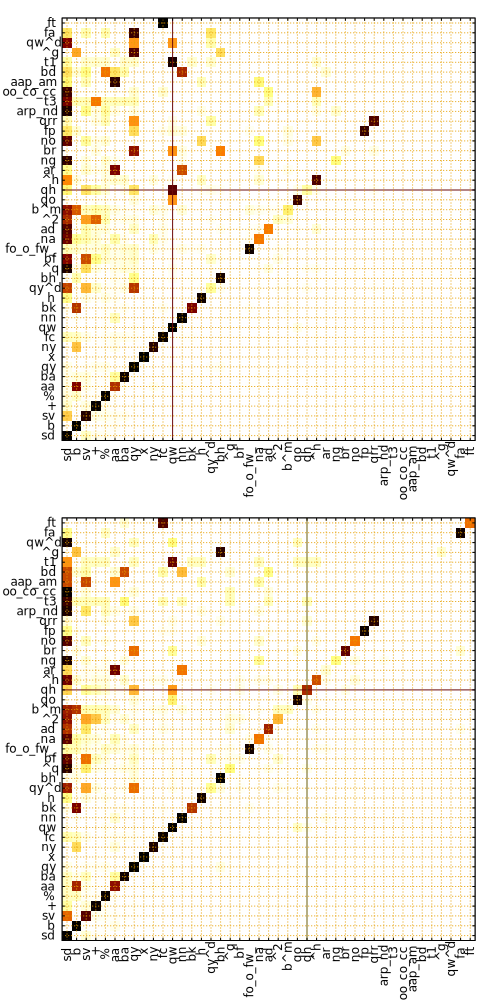
\includegraphics[width=\linewidth]{img/swda-cm.pdf}
  \caption{Confusion matrices for \texttt{BERT-NL} (top) vs \texttt{BERT-L} (bottom); SWDA corpus. Solid lines show classification improvement  of rhetorical questions.}
    \label{fig:swda-cm}
  \end{figure}

  % TODO: ^ insert SVG image!

  Confusion matrices (Figure~\ref{fig:swda-cm}) provide some food for
  thought. Most of the misclassifications fall into the majority
  classes, such as \emph{sd} (Statement-non-opinion), on left edge
  of the matrix. However, there are some important exceptions, such as
  \emph{rhetorical questions}, that are misclassified as other forms
  of questions due to their surface question-like form.  Importantly,
  laughter helps to classify rhetorical questions correctly, this is
  because in a conversation it can be used as a device to cancel
  seriousness or reduce commitment to literal meaning % sincerity
  \citep{ginzburg2015understanding,tepperman2006yeah} 
  %\todo{I actually like much more to say that it signal a clash between the literal and the intended meanning.... I think this is the basic think it does.. and then one derive the inference that the person is "not being serious"... sincerity is a big issue... I wouldn't use that word.... you know the non-bona fide stuff.... but I don't know.... I actually didn't reallu tepperman fully.. XD}.  
  Therefore,
  questions, like the one we show in example \ref{ex:rhet-qu}, are
  easier to disambiguate with laughter.
% \begin{table}
%       \small
%   \centering
%   \begin{tabularx}{\linewidth}{llL}
%     \toprule
%     Speaker & DA & Utterance \\ \midrule
%         \multicolumn{3}{c}{\emph{(Talking about hobbies)}}\\
%     B   & sd	&  Um, as far as spare time, they talked about, \\
%     B	& \% & I don't, + I think, \\
%     B	& qh & who has any spare time \texttt{<laughter>}? \\
%     A	& x & \texttt{<laughter>}.\\
%              \bottomrule
%   \end{tabularx}
%   \caption{Example from the SWDA corpus (sw3735). B's contribution \emph{qh} (Rhetorical question) is misinterpreted as \emph{qw} (Wh-question) by the BERT model without laughs in training data. }
%   \label{table:example-qh}
% \end{table}


\begin{lingex}
\item\label{ex:rhet-qu}
  \small
  \adjustbox{valign=t}{
    % \setlength\tabcolsep{1.5pt}
    \begin{tabulary}{\linewidth}{@{}>{\bf}lJ>{\em}r@{}}
      B: & Um, as far as spare time, they talked about, & Statement (n/o) \\
      B: & I don't, + I think, &  Statement (n/o) \\
       B: & who has any spare time \texttt{<laughter>}?  &  Rhetorical Quest. \\
      A: & \texttt{<laughter>}. & Non-verbal
\end{tabulary}}
\end{lingex}



  % TODO: mapping groups?

\subsection{Experiment 2: laughter and pre-training}
\label{sec:exper-2:-laught}

As previously noted, training data for BERT does not include
features specific to dialogue (e.g.\ laughs). We therefore  experiment
with a large and more dialogue-like corpus constructed from
OpenSubtitles \citep{Lison2016} (350M tokens, where 0.3\% are laughter
tokens).  We used a manually constructed list of words frequently used
to refer to laughter in subtitles and replaced every occurance of one
of these words with the special laughter token.  We then collected
every English-language subtitle file in which at least 1\% of the
utterances contained laughter (about 11\% of the total).  Because
utterances are not labelled with speaker in the OpenSubtitles corpus,
we randomly assigned a speaker token to each utterance to maintain the
format of the other dialouge corpora.

The pre-training corpus was prepared for the combined masked language
modelling and next sentence (utterance) prediction task, as described
by \citet{devlinBERTPretrainingDeep2018}.

%Here, 
We analyse how pre-training affects BERT's performance as an utterance encoder.
To do so, we consider the performance of DAR models with three different utterance encoders:
\begin{enumerate*}[i)]
\item \texttt{FT} -- pre-trained BERT with DAR fine-tuning;
\item \texttt{RI} -- randomly initialised BERT (with DAR fine-tuning);
\item \texttt{FZ} -- pre-trained BERT without fine-tuning (frozen during DAR training).
\end{enumerate*}
For the pre-trained (\texttt{FT}, \texttt{FZ}) conditions we perform two types of
pre-training:
\begin{enumerate*}[i)]
\item \texttt{OSL} -- pre-training on the portion of OpenSubtitles corpus
\item \texttt{OSNL} -- same as \texttt{OSL}, but with all the laughs removed.
\end{enumerate*}
We fine-tune and test our models on the corpora containing laughs (\texttt{L}).

%\textbf{TODO: describe the results}
We observe that dialogue pre-training improves performance of the
models. Fine-tuned models also perform better than the frozen ones
because the latter provide less opportunities for the encoder to be
trained for the specific task.

Including laughter in pre-training data improves F1 scores in most
cases, except for the SWDA in the fine-tuned condition. The difference
is especially pronounced for AMI-DA corpus in the fine-tuned condition
(4.97 p.p.\ difference in F1). The question of relevance of movies
subtitle data for either SWDA or AMI-DA can be a subject for further
study, including the types of laughs in the corpora. It might be the
case that nature of AMI-DA is congruent with those of movie
subtitles, since participants in AMI-DA basically are role-playing being in a 
focus group rather than being involved in a natural
dialogue. People might produce laughs in places only  where
they intuitively expected by them to be produced (i.e.\ humour
related), just as in scripted movie dialogues.

\begin{table}[ht]
  \small
\begin{tabularx}{\linewidth}{@{}Lrrrr@{}}
           & \multicolumn{2}{c}{\textbf{SWDA}}                          & \multicolumn{2}{c}{\textbf{AMI-DA}}                        \\ 
           & \multicolumn{1}{c}{F1} & \multicolumn{1}{c}{acc.} & \multicolumn{1}{c}{F1} & \multicolumn{1}{c}{acc.} \\
\texttt{BERT-L-FT}         & 36.75 & 76.60 & 43.37 & 64.87 \\
\bf\texttt{BERT-L+OSL-FT}  & 41.42 & 76.95 & 48.65 & 68.07 \\ 
\bf\texttt{BERT-L+OSNL-FT} & 43.71 & 77.09 & 43.68 & 64.80 \\ \hline
\bf\texttt{BERT-L+OSL-FZ}  &  9.60 & 57.67 & 17.03 & 51.03 \\ 
\bf\texttt{BERT-L+OSNL-FZ} &  7.69 & 55.29 & 16.99 & 51.46  \\ \hline
\texttt{BERT-L-RI}         & 32.18 & 73.80 & 34.88 & 60.89 \\ 
 Majority class       & 0.78  & 33.56 &  1.88 & 28.27      \\ 
    SotA              &    -  & 83.1\footnotemark & - & -  \\
\end{tabularx}
\caption{Comparison of macro-F1 and accuracy with further dialogue pre-training.  % ,
  % for the frozen (\texttt{FZ}) and fine-tuned (\texttt{FT}) conditions. \texttt{L-RI} uses a randomly initialised utterance encoder with no pre-training but with fine-tuning. Pretraining is either performed on OpenSubtitles corpus with (\texttt{OSL}) or without including laughter (\texttt{OSNL}).
\label{tab:results}}
\end{table}

\footnotetext{\citet{Kozareva2019}} 

\subsection{Experiment 3: Laughter as a non-verbal dialogue act}
\label{sec:laughter-as-non}

In this experiment, following the observations regarding the
misleading character of \emph{Non-verbal} dialogue acts, we looked at
the predictions that the model would give this class of dialogue acts
if it wasn't aware of the \emph{Non-verbal} class. To do so, we mask
the outputs of the model where the desired class was \emph{Non-verbal}
and do not backpropagate these results. We used the \texttt{BERT-L-FT}
for this experiment. After training we tested the resulting model on
the test set containing 659 non-verbal dialogue acts, 413 of which
contain laughter.

For 314 (76\%) of such dialogue acts the model has predicted the
\emph{Acknowledge (Backchannel)} class and for 46 (11\%) ---
continuations of the previous DA by the same speaker. The rest were
classified as either something uninformative (the \emph{Abandoned or
  Turn-Exit or Uninterpretable} class) or, from manual observation,
clearly unrelated.

\emph{Acknowledge (Backchannel)} can cover some uses of laughter, for
instance, to show to the interlocutor acknowledgement of their
contribution, implying the appreciation of an incongruity, and
inviting continuation (functioning simultaneously as a continuer and
assessment feedback
\citep{schegloff1982discourse}), as in example~\ref{ex:fish}.

\begin{lingex}
  \small
\item\label{ex:fish}  \small
  %From sw2290.
  (We mark continuations of the previous DA by the same speaker with a plus, and indicate misclassified dialogue acts with a star. Laughs shown in bold constitute \emph{Non-verbal} dialogue acts)\\
    % \adjustbox{valign=t}{
    % \setlength\tabcolsep{2pt}
    \begin{tabulary}{\linewidth}{@{}>{\bf}lJ>{\em}r@{}}
B: & Everyone on the boat was catching snapper, snappers except guess who. & Statement (n/o)  \\ 
A: & <laughter> It had to be you. & Summ./reform.  \\
B: & <laughter> I ca-, I, - & Uninterpretable \\
A: & Couldn't catch one to save your life. Huh. & %Summarize/reformulate $\to$
Backchannel$^*$\\
B: & That's right, & Agree/Accept \\
B: & I would go from one side of the boat to the other, & Statement (n/o) \\
B: & and, uh, & $+$ \\
A: & \bf <laughter>. &Backchannel\\
B: & the, uh, the party boat captain could not understand, you know, & $+$ \\
B: & he even, even he started baiting my hook <laughter>, & Statement (n/o) \\
A: & \bf <laughter>. &Backchannel\\
B: & and holding, holding the, uh, the fishing rod. & $+$\\
A: & How funny, & Appreciation \\
% A & just hoping maybe, he could pull <laughter>. - & %Summarize/reformulate $\to$
% Statement (n/o)$^*$ \\
% B & Right, <laughter> & %aa $\to$
% Backchannel$^*$ \\
% B & and it was, it was really, really, really bad. & Statement (n/o)  
\end{tabulary}
% }
\end{lingex}

Nevertheless, these two cases clearly cannot account for all the
examples discussed in the literature (e.g.\ standalone uses of
laughter as signal of disbelief or negative response to a polar
question \citealp{ginzburg2020laughter}) and above in
Sec.~\ref{sec:observations}. Future models will therefore require a
manual assignment of meaningful dialogue acts to standalone laughs.



% \begin{table}
%   \centering
%   \begin{tabularx}{\linewidth}{@{}Ll@{}}
%     \toprule
%     Assigned class &  \\\midrule
%     Backchannel   & 314 \\
%     Other & 42 \\
%     Continuer (preceding DA) & 46 \\
%     Quotation & 8 \\
%     Collaborative completion & 2 \\
%     Conventional-closing & 1 \\\midrule
%     TOTAL & 413 \\
%     \bottomrule
%   \end{tabularx}
%   \caption{Distribution of model predictions for dialogue acts annotated as \emph{non-verbal}. }
%   \label{tab:nv-results}
% \end{table}

% - inconclusive
% not bad to consider as backchannels. But not the same as the examples above for standalone: glossa examples
% - signalling understanding
% - enriching this understanding with emotional appraisal
% we need an annotation

\section{Discussion}
\label{sec:discussion}
The implications of the results obtained are twofold: showing that
laughter can help a computational model to attribute meaning to an
utterance and help with pragmatic disambiguation, and consequently
stressing once again the need for integrating laughter (and other
non-verbal social signals) in any framework aimed to model meaning in
interaction \citep{ginzburg2020laughter,Maraev.Mazzocconi.Howes.Ginzburg_ISCA_2018}. % TODO: and, in final version add LACATODA

% \subsection{Laughter and pragmatic disambiguation}
% \label{sec:laught-dial-acts}

Our results provide further evidence
(e.g. \citet{torres1997modeling,gazelaughter}) for the fact that
non-verbal behaviours are tightly related to the dialogue information
structure, propositional content and  dialogue act performed by
utterances.
Laughter, along with other non-verbal social signals, can constitute a
dialogue act in itself conveying meaning and affecting the unfolding
 dialogue \citep{bavelas2000visible,ginzburg2020laughter}.


% \subsection{Laughter and dialogue act recognition task}
% \label{sec:dar-task}
In this work we have shown that laughter is a valuable cue for DAR
task. We believe that in our conversations laughter is informative
about interlocutors' emotional and cognitive appraisals of events and
communicative intents. %\citep{mazzocconi2019phd}. 
Therefore, it should not come as a surprise
%\todo{mmm... maybe I do not love it... I mean it super cool!!! maybe say it is not surprise makes it a bit less cool... should we rather say we think that's why it helps also the model? } 
that laughter
acts as a cue in a computational model.

On the question of laughter impact on the dialogue act recognition
(DAR) task, this study found that laughter is more helpful in SWDA
corpus than in AMI-DA.  Due to the nature of interactions over the
phone, SWDA dialogue participants can not rely on visual signals, such
as gestures and facial expressions.  Our results support the
hypothesis that in SWDA, vocalizations such as laughter are more
pronounced and therefore more helpful in disambiguating dialogue acts.
This may also explain why our best models perform better on SWDA:
more of the information that interlocutors and dialogue act annotators
rely on is present in SWDA transcripts, whereas AMI-DA annotators receive
clear instructions to pay attention to the videos
\citep{GuidelinesDialogueAct2005}.  This finding is consistent with
that of \citet{bavelas2008gesturing} who demonstrate that in
face-to-face dialogue, visual components, such as gestures, can convey
information that is independent from what is conveyed by speech.

Laughter can be used to mark the presence of an incongruity between
what is said and what is intended, coined as \emph{pragmatic
  incongruity} by \citet{mazzocconiTAC}. In those cases laughter is
especially valuable for disambiguating between literal and non-literal
meaning, as we have shown for rhetorical questions, a task which is
still a struggle for most NLP models and dialogue systems.

There is abundant room for further progress in determining how other speech-related information, such as prosody and disfluencies, can be incorporated into a DAR model.
\citet{stolckeDialogueActModeling2000} showed that dialogue acts can have specific prosodic manifestations that can be used to improve DAR.
Furthermore, in relation to laughter, its form (duration, arousal, overlap with speech) can be informative about its function and position w.r.t.\ the laughable \citep{tian2016we,mazzocconi2019phd}.
Incorporating such information is crucial if models pre-trained on large-scale text corpora are to be adapted for use in dialogue applications.



% - communicative intentions (not just turn and "sequencing") 
% - non-literal meaning (also supported by the BERT model)
% - not being "just" non-verbal! Bavelas!

% TODO: what about more appropriate dialogue act annotation schemes?


% \section*{Acknowledgments}

% The acknowledgments should go immediately before the references. Do not number the acknowledgments section.
% \textbf{Do not include this section when submitting your paper for review.}

\bibliographystyle{acl_natbib}
\bibliography{semdial}
\appendix
\onecolumn
\section{Supplementary materials}\label{sec:suppl}

\subsection{Collocations of laughs and dialogue acts}
\label{sec:app:da-svd}


\begin{figure*}[h!]
  \centering
  \fontsize{6}{10}\selectfont
  \sffamily
  \includesvg[width=\linewidth]{img/da-svd-verbal}
  \caption{Singular value decomposition of pentagonal representations of dialogue acts. For a selection of dialogue acts (in purple) we depict their pentagon representations.}
    \label{fig:da-svd}
\end{figure*}

\pagebreak

\begin{figure*}[h!]
\subsection{Model performance in DAR task}
\label{sec:app:bert}

  \centering
  \includegraphics[width=\linewidth]{img/SWDA-bertLvsNL.pdf}
  \includegraphics[width=\linewidth]{img/AMI-DA-bertLvsNL.pdf}
  \caption{Change in accuracy for each dialogue act (\texttt{BERT-NL} vs \texttt{BERT-L}). Positive changes when adding laughter (\texttt{BERT-L}) are shown in blue. Vertical bars indicate how often dialogue act is associated with laughter. Top chart: SWDA, Bottom chart: AMI-DA. }
    \label{fig:by-da}
\end{figure*}


\end{document}